\documentclass[10pt]{article}

\usepackage[T1]{fontenc}
\usepackage{graphicx}	% Including figure files
\usepackage{amsmath}	% Advanced maths commands
\usepackage{amssymb}	% Extra maths symbols
\usepackage{physics}
\usepackage{natbib}
\usepackage[margin=1in]{geometry}
\usepackage{hyperref}

\renewcommand{\Re}{\mathrm{Re}}
\newcommand{\Dv}[2]{\frac{D#1}{D#2}}
\newcommand{\lint}{\int\limits}

\title{Stably stratified low-Pr turbulence:\\ The Computational Lab Notebook}

\author{
    Ben Goldman,$^{1}$\thanks{E-mail: bog2101@columbia.edu}
    Valentin Skoutinev,$^{1}$
    \\
    % List of institutions
    $^{1}$Department of Physics, Columbia University
}

\begin{document}
\label{firstpage}
\maketitle

% Abstract of the paper
\begin{abstract}
    This is the lab notebook for this summer's project! Here I'll state the research question and its answer as the research progresses.
\end{abstract}

\section{Introduction}

Here I'll do my review of literature, and show how the research question follows from overall field goals and past discoveries.

\section{Methods, Observations, Simulations etc.}

\subsection{Kelvin-Helmholtz linear perturbation growth}

\subsubsection{Analytical hypothesis}
This analysis follows \citet{kundu2004}
Assume a doubly periodic box of fluid, where above $z=0$ we have a flow velocity $U_1$ and density $\rho_1$ and below $z=0$ we have flow velocity $U_2$ and density $\rho_2$. We approximate the flow as inviscid, i.e. $\Re \approx \infty$. We represent the boundary between the separate layers with the function $z = \zeta(x, y)$ Assume that the fluid is incompressible, meaning that the flow velocity is the gradient of some potential function. The symbol ~ will indicate perturbed quantities. We can represent the flow potential as the sum of its background state ($\grad U_1$ and $\grad U_2$) and a perturbation $\vec{u}_1 = (u_1, v_1, w_1)$ and $\vec{u}_2 = (u_2, v_2, w_2)$ with
\begin{align}
    \tilde{u}_1 = U_1 + \vec{u}_1 \\
    \tilde{u}_2 = U_2 + \vec{u}_2
\end{align}
that are associated with potentials
\begin{align}
    \tilde{\phi}_1 = U_1x + \phi_1 \\
    \tilde{\phi}_2 = U_2x + \phi_2.
\end{align}

The flow is incompressible, so we have
\begin{align}
    \div{\tilde{u}_1} = \laplacian \tilde\phi_1 = 0 \qq{and} \div\tilde u_2 = \laplacian \tilde\phi_2,
\end{align}
but since the background flow is already incompressible, we also have
\begin{align}
    \laplacian\phi_1 = 0 \qq{and} \laplacian\phi_2 = 0. \label{eq:lap}
\end{align}

The perturbed flow only makes physical sense when the perturbation drops off far from the interface. Therefore, we have the boundary conditions
\[\mqty{\phi_1 \to 0\\\phi_2\to 0} \qq{as} z\to\infty.\]
Since the interface at $z=\zeta$ divides the two flows, we know that "particles at the interface must move with the interface.", imposing the requirement that
\[\tilde{u}_1 = \pdv{\phi_1}{z} = \Dv{\zeta}{t} \qq{at} z = \zeta\]
which expands to
\begin{align}
    \pdv{\phi_1}{z} & = \pdv{\zeta}{t} + (\tilde{u}_1 \vdot \grad)\zeta \\
                    & = \pdv{\zeta}{t} + (U_1 + u_1)\pdv{\zeta}{x} + v_1\pdv{\zeta}{y} \\
                    & = \pdv{\zeta}{t} + U_1\pdv{\zeta}{x} + u_1\pdv{\zeta}{x} + v_1\pdv{\zeta}{y} \qq{at} z = \zeta.
\end{align}
Since the flow is 2-dimensional, we have $v_1 = 0$. We linearize this equation by applying it at $z = 0 \approx \zeta$ and dropping terms that are second-order in small quantities (i.e. $u_1\pdv{\zeta}{t}$). Repeating this process on the particles below the boundary produces the conditions
\[\mqty{
        \pdv{\phi_1}{t} & = \pdv{\zeta}{t} + U_1\pdv{\zeta}{x} \\
    \pdv{\phi_2}{t} & = \pdv{\zeta}{t} + U_2\pdv{\zeta}{x}} \qq{at} z = 0
\]

Next, consider the pressure of the fluids at the boundary $\zeta$, which must be equal. We can study this using the Bernoulli equations for unsteady inviscid irrotational flow, 

\begin{align}
    \pdv{\tilde\phi_1}{t} + \frac{1}{2}(\grad\tilde\phi_1)^2 + \frac{\tilde p_1}{\rho_1} + gz = C_1 \label{eq:ber1} \\
    \pdv{\tilde\phi_2}{t} + \frac{1}{2}(\grad\tilde\phi_2)^2 + \frac{\tilde p_2}{\rho_2} + gz = C_2 \label{eq:ber2}.
\end{align}
We can eliminate the unknowns $C_1$ and $C_2$ by considering the initial state of this equation at the interface given a perturbation of zero amplitude, meaning we have $z = 0$ and $\pdv{\tilde\phi_1}{t} = \pdv{\tilde\phi_2}{t} = 0$ with $\tilde p_1 = \tilde p_2 = p_1 = p_2$. Under these conditions, the above equations simplify to
\begin{align}
    \frac{1}{2}U_1^2 + \frac{p_1}{\rho_1} = C_1 & \implies p_1 = \rho_1\qty(C_1 - \frac{1}{2}U_1^2) \label{eq:cc1} \\
    \frac{1}{2}U_2^2 + \frac{p_2}{\rho_2} = C_2 & \implies p_2 = \rho_2\qty(C_2 - \frac{1}{2}U_2^2) \label{eq:cc2} \\
    \rho_1\qty(C_1 - \frac{1}{2}U_1^2) & = \rho_2\qty(C_2 - \frac{1}{2}U_2^2) \label{eq:cc}.
\end{align}

Solving equations \eqref{eq:ber1} and \eqref{eq:ber2} for pressure and equating them produces
\begin{align}
    \begin{split}
        \tilde p_1 = \tilde p_2 & = \rho_1C_1 - \rho_1g\zeta - \frac{\rho_1}{2}[(U_1 + u_1)^2 + v_1^2 + w_1^2] - \rho_1\pdv{\phi_1}{t} \\
                                & = \rho_2C_2 - \rho_2g\zeta - \frac{\rho_2}{2}[(U_2 + u_2)^2 + v_2^2 + w_2^2] - \rho_2\pdv{\phi_2}{t}
    \end{split}
\end{align}
to which we can now add \eqref{eq:cc},
\begin{align}
    \begin{split}
        \frac{\rho_1}{2}U_1^2 & - \rho_1g\zeta - \frac{\rho_1}{2}[(U_1 + u_1)^2 + w_1^2] - \rho_1\pdv{\phi_1}{t} \\
                              & = \frac{\rho_2}{2}U_2^2 - \rho_2g\zeta - \frac{\rho_2}{2}[(U_2 + u_2)^2 + w_2^2] - \rho_2\pdv{\phi_2}{t},
    \end{split}
\end{align}
where I drop $v$'s since the flow is 2-dimensional. The above expands to
\begin{align}
    \begin{split}
        \frac{\rho_1}{2}U_1^2 & - \rho_1g\zeta - \frac{\rho_1}{2}[2U_1u_1 + U_1^2 + u_1^2 + w_1^2] - \rho_1\pdv{\phi_1}{t} \\
                              & = \frac{\rho_2}{2}U_2^2 - \rho_2g\zeta - \frac{\rho_2}{2}[2U_2u_2 + U_2^2 + u_2^2 + w_2^2] - \rho_2\pdv{\phi_2}{t},
    \end{split}
\end{align}
where the terms $u^2$ and $w^2$ are negligible to first order, the $U^2$'s cancel, and we approximate $z = \zeta = 0$ yielding
\begin{align}
    \rho_1\qty(g\zeta + U_1u_1 + \pdv{\phi_1}{t}) = \rho_2\qty(g\zeta + U_2u_2 + \pdv{\phi_2}{t}),
\end{align}
which, in terms of potential, is
\begin{align}
    \rho_1\qty(g\zeta + U_1\pdv{\phi_1}{x} + \pdv{\phi_1}{t}) = \rho_2\qty(g\zeta + U_2\pdv{\phi_2}{x} + \pdv{\phi_2}{t}) \qq{at} z = 0 \label{eq:ber3}.
\end{align}

Approximate the variables $\phi_1$, $\phi_2$, $\zeta$ as sinusoidal normal modes, built like
\begin{align}
    \zeta & = \hat\zeta e^{ik(x-ct)} \\
    \phi_1 & = \hat\phi_1 e^{ik(x-ct)} \\
    \phi_2 & = \hat\phi_2 e^{ik(x-ct)}
\end{align}
for unknown amplitudes $\hat\phi_1(z), \hat\phi_2(z), \hat\zeta$ the Laplace equation \eqref{eq:lap} demands solutions for which we have
\begin{align}
    \hat\phi_1 = Ae^{\pm kz} \\
    \hat\phi_2 = Be^{\pm kz}
\end{align}
where we can drop the positive exponential for $\hat\phi_1$ and the negative exponential in $\hat\phi_2$ since these would violate the condition that deviations drop off at long distance. Now, I substitute these solutions into equations \eqref{eq:cc1} and \eqref{eq:cc2} to solve for $A$ and $B$:
\begin{align}
    -Ake^{-kz}e^{ik(x-ct)} & = -\hat\zeta ikce^{ix(x-ct)} + \zeta ikU_1e^{ik(x-ct)} \qq{at} z = 0 \nonumber \\
    A & = \hat\zeta i(c-U_1) \\
    Bke^{k-}e^{ik(x-ct)} & = -\hat\zeta ikce^{ik(x-ct)} + \hat\zeta ikU_2e^{ik(x-ct)} \qq{at} z = 0 \nonumber \\
    B & = -\hat\zeta i(c - U_2).
\end{align}
Throwing the solutions into \eqref{eq:ber3} then produces
\begin{align}
    p_1 & = \rho_1\qty(g\hat\zeta e^{ik(x-ct)} + \hat\phi_1ikU_1e^{ik(x-ct)} - \hat\phi_1ikce^{ik(x-ct)}) \\
        & = \rho_1e^{ik(x-ct)}\qty(g\hat\zeta + \hat\phi_1ikU_1 - \hat\phi_1ikc) \nonumber \\
    = p_2 & = \rho_2\qty(g\hat\zeta e^{ik(x-ct)} + \hat\phi_2ikU_2e^{ik(x-ct)} - \hat\phi_2ikce^{ik(x-ct)}) \nonumber \\
          & = \rho_2e^{ik(x-ct)}\qty(g\hat\zeta + \hat\phi_2ikU_2 - \hat\phi_2ikc),
\end{align}
but since $\hat\phi_1 = A$ and $\hat\phi_2 = B$ at $z = 0$, this implies
\begin{align}
    \rho_1\qty(g\hat\zeta + Aik(U_1 - c)) = \rho_2\qty(g\hat\zeta + Bik(U_2 - c)).
\end{align}
After substituting $A$ and $B$ into this, we have
\begin{align}
    \rho_1\qty(g\hat\zeta + \hat\zeta k(U_1 - c)(U_1 - c)) = \rho_2\qty(g\hat\zeta - \hat\zeta k(U_2 - c)(U_2 - c)),
\end{align}
which is equivalent to
\begin{align}
    g(\rho_1 - \rho_2) = k\qty(\rho_1(U_1 - c)^2 + \rho_2(U_2-c)^2).
\end{align}
In the case of a vortex sheet, we have $\rho_1 = \rho_2$, so the above simplifies to
\begin{align}
    0 = k\qty(\rho_1(U_1 - c)^2 + \rho_2(U_2-c)^2).
\end{align}
Now, let us consider the case in which $U_1 = -U_2 = U$, which can be trivially achieved for any KH flow by performing a Galilean transformation by the average of $U_1$ and $U_2$. The above further simplifies down to
\begin{align}
    0 = k\qty(\rho_1(U - c)^2 + \rho_2(U + c)^2) = kU^2 + kc^2 \implies c^2 = -U^2
\end{align}

Now, to obtain the growth rate of a sinusoidal perturbation to the vortex sheet, take the second time-derivative of one of the potentials and substitute $c^2$,
\begin{align}
    \dv[2]{\phi_1}{t} = -\hat\phi_1k^2c^2e^{ik(x-ct)} = -k^2c^2\phi_1 = k^2U^2\phi_1
\end{align}

Therefore, we see that perturbations of wavenumber $k$ to a vortex sheet grow at a rate proportional to the product of the wavenumber and half the difference in shear flow velocities.

\subsubsection{attempted experimental verification}

We approximate the solution by using a pseudo-spectral DNS solver \citep{mortensen2016}, calculated over a doubly-periodic (2-dimensional) domain of width and height $L$ with a mesh size of $512\times512$. A KH instability is initialized with horizontal shear flow given by
\[U_x = \tanh(\frac{\frac{2\pi z}{L} - \pi}{\delta})\]
where $\delta \sim 0.01L$. We perturb this background flow with an initial sinusoidal perturbation of wavenumber $k$ and initial amplitude $A$ that decreases exponentially  from the shear boundary,
\[U_z = A\sin(\frac{2\pi k x}{L})e^{((\frac{2\pi z}{L}-\pi)/k)^2}\]
where $A \sim 0.001\times \frac{2\pi}{L}$. We initialize uniform pressure and density. The simulation is run for $k = 1, 2, \dots, 10$ for $0 \leq t \leq 0.5$ with a 4th order Runge-Kutta time-step with a maximum step-size of $0.0001$.

I approximate the amplitude of a perturbation with the standard deviation of the vertical velocity field, normalized by $\sqrt{2}$. The growth rate of perturbations is found by fitting the logarithm of the amplitude  to a linear equation during its linear growth phase. We find a linear relationship between the wavenumber and the growth rate, with a proportionality constant of $1$, as shown in \ref{fig:1}, for the first 8 wavenumbers. The regression slope decreases to $0.85$ when wavenumbers 9 and 10 are included, which we attribute to numerical errors at insufficient resolution.
\begin{figure}
    \centering
    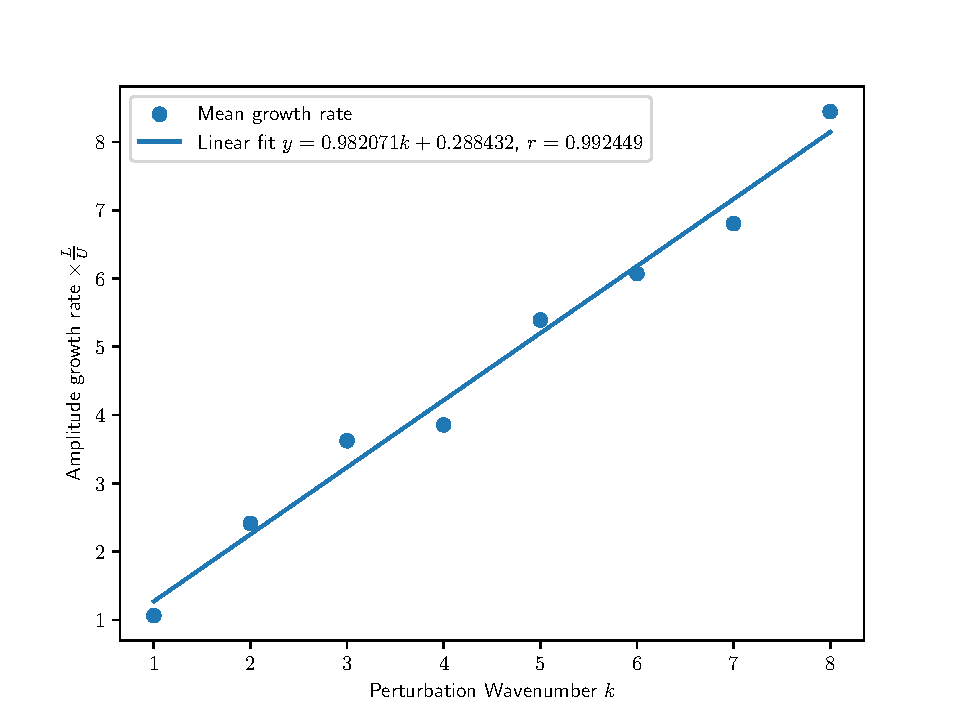
\includegraphics[width=\columnwidth]{KH1.pdf}
    \caption{KH Growth rate vs wavenumber}
    \label{fig:1}
\end{figure}

\subsection{Arbitrary Horizontal Stratification}

We have a flow with the following properties,
\[\tilde{u} = \mqty[U + u \\ 0 \\ w]\ \quad \tilde{p} = P + p \quad \tilde\rho = \bar\rho + \rho,\]
where a tilde indicates a total quantity, decomposed into background fields and fluctuation fields. We begin with the Boussinesq equations (ignoring thermal expansion),
\begin{align}
    \pdv{\tilde{u}}{t} + \tilde{u}\vdot\grad\tilde{u} & = -\frac{1}{\rho_0}\pdv{\tilde{p}}{x} + \nu\laplacian\tilde{u} \\
    \pdv{w}{t} + w\vdot\grad w & = -\frac{1}{\rho_0}\pdv{\tilde{P}}{z} - \frac{\rho g}{\rho_0} = \nu\laplacian w \\
    \pdv{\tilde{u}}{x} + \pdv{w}{z} & = 0
\end{align}
these can notationally be combined into
\begin{align}
    \pdv{t}(U_i + u_i) + (U_j + u_j)\pdv{x_j}(U_i + u_i) = -\frac{g}{\rho_0}(\bar\rho + \rho)\delta_{i3} - \frac{1}{\rho_0}\pdv{x_i}(P + p)
\end{align}
where total quantities have been decomposed into background and variable fields, and we drop the viscosity term. For the background flow, since it's not time-dependent, we know that it's pressure is in equilibrium, given by,
\begin{align}
    0 = -\frac{g\bar\rho}{\rho_0}\delta_{i3} - \frac{1}{\rho_0}\pdv{P}{x_i}.
\end{align}
Now, I subtract the above two equations, yielding
\begin{align}
    \pdv{t}(U_i + u_i) + (U_j + u_j)\pdv{x_j}(U_i + u_i) = \frac{g\rho}{\rho_0}\delta{i3} - \frac{1}{\rho_0}\pdv{p}{x_i}.
\end{align}
Since the background flow is steady, we have $\pdv{U_i}{t} = 0$. Next, we drop nonlinear small terms $u_j\pdv{u_i}{x_j}$, so we have,
\begin{align}
    \pdv{u_i}{t} + u_j\pdv{U_i}{x_j} + u_j\pdv{u_i}{x_j} = -\frac{g\rho}{\rho_0}\delta_{i3} - \frac{1}{\rho_i}\pdv{p}{x_j}.
\end{align}
Extracting the $x$ and $z$ terms from this formula gives
\begin{align}
    \pdv{u}{t} + w\pdv{U}{z} + U\pdv{u}{x} & = -\frac{1}{\rho_0}\pdv{p}{x} \\
    \pdv{w}{t} + U\pdv{w}{x} & = -\frac{g\rho}{\rho_0} - \frac{1}{\rho_0}\pdv{p}{z}
\end{align}
Since we feel like neglecting density diffusion here, we know that density is conserved along particle paths, i.e.
\begin{align}
    \frac{D\tilde\rho}{Dt} = 0 & = \pdv{\tilde\rho}{t} + \tilde{u}\vdot\grad\tilde\rho \\
                               & = \pdv{t}(\bar\rho + \rho) + (U + u)\pdv{x}(\bar\rho + \rho) + w\pdv{z}(\bar\rho + \rho)
\end{align}
After dropping nonlinear terms, this reduces to
\begin{align}
    \pdv{\rho}{t} + U\pdv{\rho}{x} - \frac{\rho_0N^2w}{g} = 0
\end{align}
where $N^2 \equiv -\frac{g}{\rho_0}\pdv{\bar\rho}{z}$ is the Brunt V\"ais\"al\"a frequency.

We can account for the continuity equation by making a streamfunction $\psi$ with
\begin{align}
    u = \pdv{\psi}{z} \qq{and} w = -\pdv{\psi}{x},
\end{align}
or, in the more terse subscript notation, $u = \psi_z$ and $w = -\psi_x$. We can now use this streamfunction to solve the system of $u$, $v$, $\rho$, and $p$. Substituting $\psi$ into this system gives the set
\begin{align}
    \psi_{zt} -\psi_zU_z + U\psi_{zx} & = -\frac{1}{\rho_0}p_x \\
    -\psi_{xt} - U\psi_{xx} & = -\frac{g\rho}{\rho_0} - \frac{1}{\rho_00}p_z \\
    \rho_t + U\rho_x + \frac{\rho_0N^2}{g}\psi_x & = 0
\end{align}

Like before, a perturbed solution can be obtained by using complex exponential normal modes,
\begin{align}
    \rho & = \hat\rho(z)e^{ik(x-ct)} \\
    p & = \hat{p}(z)e^{ik(x-ct)} \\
    \psi & = \hat\psi(z)e^{ik(x-ct)},
\end{align}
where quantities wearing a hat are complex amplitudes dependent only on $z$, and $c$ is a complex phase speed, indicating spatial wave propagation and exponential growth over time. Substituting these and their derivatives into our PDE system gets us the following linear equations,
\begin{align}
    -\hat\psi_zikce^{ik(x-ct)} - \hat\psi U_z ike^{ik(x-ct)} + \hat\psi_zikUe^{ik(x-ct)} = -\frac{1}{\rho_0}\hat{p}ike^{ik(x-ct)} \\
    -\hat\psi ck^2e^{ik(x-ct)} + \hat\psi Uk^2e^{ik(x-ct)} = -\frac{g}{\rho_0}\hat\rho e^{ik(x-ct} - \frac{1}{\rho_0}\hat{p}_ze^{ik(x-ct)} \\
    -\hat\rho ikce^{ik(x-ct)} + \hat\rho Uike^{ik(x-ct)} + \frac{\rho_0N^2}{g}\hat\psi ike^{ik(x-ct)},
\end{align}
which each simplify to
\begin{align}
    (U-c)\hat\psi_z - U_z\hat\psi = \frac{1}{\rho_0}\hat{p} \\
    k^2(U-c)\hat\psi = -\frac{g}{\rho_0}\hat\rho - \frac{1}{\rho_0}\hat\rho_z \\
    (U-c)\hat\rho + \frac{\rho_0N^2}{g}\hat\psi = 0.
\end{align}
Taking the partial derivative of the first equation with respect to $z$ and then adding that to the second and third equations eventually makes
\begin{align}
    (\hat\psi_{zz} - \hat\psi k^2)(U-c) - \hat\psi U_{zz} + \hat\psi\frac{N^2}{U-c} = 0
\end{align}
which is called the Taylor-Goldstein equation. It has the boundary conditions that the flow is zero at the edges of the domain. For a rectangle, we have $\hat\psi(0) = \hat\psi(d) = 0$ I'm not too familiar with complex variables but apparently because its complex conjugate is also a valid solution, for every value of $c$ that satisfies the equation, we have a corresponding solution with $c^*$, the complex conjugate. This means that even if for some stable solution $c = c_r + ic_i$ with $c_i > 0$ we have an unstable solution with $c_i < 0$. Therefore, stable solutions are only guranteed if $c_i = 0$ exactly. This leads us to develop a useful restriction on which flows can guarantee stability. Define the helpful substitution
\begin{align}
    \phi \equiv \frac{\hat\psi}{\sqrt{U-c}} \qq{or} \hat\psi = \psi\sqrt{U-c}
\end{align}
with the first and second $z$-derivatives
\begin{align}
    \hat\psi_z & = \phi_z\sqrt{U-c} + \frac{\phi U_z}{2\sqrt{U-c}} \\
    \hat\psi_{zz} & = \phi_{zz}\sqrt{U-c} + \frac{U_z\phi_z + \frac{1}{2}\phi U_{zz}}{\sqrt{U-c}} - \frac{\phi U_z^2}{\sqrt{U-c}^3}
\end{align}

Substituting these into the Taylor-Goldstein equation produces
\begin{multline}
    (U-c)\qty(\sqrt{U-c}\phi_{zz} + \frac{U_z\phi_z + \frac{1}{2}\phi U_{zz}}{\sqrt{U-c}} - \frac{U_z^2\phi}{4\sqrt{U-c}^3} - k^2\phi\sqrt{U-c}) \\ - U_{zz}\phi\sqrt{U-c} + \frac{N^2\phi}{\sqrt{U-c}} = 0
\end{multline}
which simplifies to
\begin{align}
    \dv{z}[\phi_z(U-c)] - \phi\qty(\frac{1}{2}U_{zz} + k^2(U-c) + \frac{\frac{1}{4}U_z^2-N^2}{U-c}) = 0
\end{align}
we then multiply both sides by the complex conjugate of $\phi$, $\phi^*$, and integrate from $0$ to $d$,
\begin{align}
    \lint_0^d\dv{z}[(U-c)\phi_z]\phi^*\dd{z} = \lint_0^d\dv{z}[(U-c)\phi_z\phi^*] - (U-c)\phi_z\phi^*_z\dd{z}
\end{align}
where the right-hand-side uses integration by parts. One can show that this is equivalent to
\begin{align}
    \lint_0^d\frac{N^2 - U_z^2/4}{U-c}\dd{z} = \lint_0^d(U-c)\qty(\abs{\phi_z}^2 + k^2\abs{\phi}^2)\dd{z} + \frac{1}{2}\lint_0^dU_{zz}\abs{\phi}^2\dd{z}. \label{eq:int1}
\end{align}
Observe that since $U+c$ is really $U + c_r + ic_i$, where $U$, $c_r$, and $c_i$ are all real, we can manipulate the identity $(U+c)(U+c)^* = \abs{U+c}^2$ into
\begin{align}
    \frac{1}{U-c} = \frac{(U-c)^*}{\abs{U-c}^2} = \frac{U-c_r+ic_i}{\abs{U-c}^2}
\end{align}
whose imaginary part is
\begin{align}
    \Im\frac{1}{U-c} = \frac{c_i}{\abs{U-c}^2}
\end{align}
which we can use to take the imaginary part of equation \eqref{eq:int1}, producing
\begin{align}
    c_i\lint_0^d\frac{N^2 - U_z^2/4}{\abs{U-c}^2}\dd{z} = -c_i\lint_0^d\abs{\phi_z}^2 + k^2\abs{\phi}^2\dd{z},
\end{align}
where the former second right-hand-side term is purely real, so it drops out. The right-hand-side of the above must bear the opposite sign to $c_i$, because the integrand is definitely positive. On the other hand, the left-hand-side is positive for positive $c_i$ iff (if and only if) we have $N^2 > U_z^2/4$. Therefore, when this is the case, we necessarily have $c_i = 0$, implying that the flow is stable. This is the Richardson Number Criterion.

\subsubsection{Howard's Semicircle Theorem}
I have a derivation of this in my paper notebook, but I feel it's more pressing to move on to turbulence. In any case, the main result is that in the problem outlined below, we have
\begin{align}
    U_{\mathrm{min}} < c_r < U_{\mathrm{max}} \qq{and} kc_i < \frac{k}{2}(U_{\mathrm{max}} - U_{\mathrm{min}})
\end{align}
In words, this means that the horizontal velocity of linear wave propagation must be within the range of velocities in the background flow, and that the exponential growth of unstable linear waves is limited by the range of velocities in the background flow. For example, for the Kelvin-Helmholtz instability of uniform density derived above, we have $U_{\mathrm{min}} = -1$ and $U_{\mathrm{max}} = 1$, and we found $c_r = 0$ and $c_i = 1$ This is consistent with Howard's Semicircle Theorem.

\subsection{Turbulence}

\subsubsection{Energy Budget and Scaling Conclusions}
Here, we are also Following \citet{kundu2004}.
Let's say we have a turbulent flow given by the variables
\begin{align}
    \tilde{u} & = \vec{U} + \vec{u} = \mqty[U\\V\\W] + \mqty[u\\v\\w] \qq{or} \tilde{u} = U_i + u_i, \\
    \tilde{P} & = P + p, \\
    \tilde{T} & = \bar{T} + T',
\end{align}
where the first term is mean flow, and the second is turbulent flow, such that $\overline{u} = 0$, where $\overline{(\cdot)}$ denotes an average.

We can decompose the Boussinesq set into mean and turbulent parts. The mean and turbulent continuity equations become
\begin{align}
    \pdv{U_i}{x_i} = 0 \qq{and} \pdv{u_i}{x_i} = 0.
\end{align}
The momentum equation is slightly more complicated. For the mean flow, we have
\begin{align}
    \frac{DU_i}{Dt} = -\frac{1}{\rho_0}\pdv{\bar\tau_{ij}}{x_j} - g[1-\alpha(\bar{T} - T_0)]\delta_{i3}
\end{align}
where $\bar\tau_{ij}$ is given by
\begin{align}
    \bar\tau_{ij} = -P\delta_{ij} + \mu\qty(\pdv{U_i}{x_j} + \pdv{U_j}{x_i}) - \rho_0\overline{u_iu_j}
\end{align}
By multiplying this by $U_i$, we can obtain the energy budget for the mean flow. First, define the mean strain rate
\begin{align}
    E_{ij} = \frac{1}{2}\qty(\pdv{U_i}{x_j} + \pdv{U_j}{x_i})
\end{align}
to indicate the rate at which a parcel (here usually a vortex) gets stretched or deformed. The kinetic energy budget comes out to
\begin{align}
    \frac{D}{Dt}\qty(\frac{1}{2}U_i^2) & = \pdv{x_j}\qty(-\frac{PU_j}{\rho_0} + 2\nu U_iE_{ij} - \overline{u_iu_j}U_i) - 2\nu E_{ij}E_{ij} + \overline{u_iu_j}\pdv{U_i}{x_j} - \frac{g}{\rho_0}\bar\rho U_3
\end{align}
By performing a surface integral and applying Gauss's theorem, one can show that the first three terms on the right-hand-side do not affect the total energy; they only transport energy within a volume. The fifth term describes the total energy transferred by vortex stretching from the mean flow to the turbulent flow. This term will be negative because it transfers energy to lower length scales. The sixth term captures the transfer between kinetic and gravitational potential energy (analogous to $W_{\text{gravity}} = mgv_y$ for a free particle). For the mean flow, we expect to have $\Re \gg 1$. Additionally, since the mean strain rate term $\nu E_{ij}^2$ is of order $\nu U^2/L^2$, while the turbulent loss term, $\overline{u_iu_j}\pdv{U_i}{x_j}$ is of order $U^3/L$, we expect the fourth term, the one that captures the role of viscous dissipation to be negligible relative to the others for the mean flow.

For the turbulent component, we will be using the turbulent strain rate tensor,
\begin{align}
    e_{ij} = \frac{1}{2}\qty(\pdv{u_i}{x_j} + \pdv{u_j}{x_i}),
\end{align}
and one can show that the averaged kinetic energy equation is
\begin{align}
    \frac{D}{Dt}\overline{\qty(\frac{1}{2}u_i^2)} = -\pdv{x_j}\qty(\frac{1}{\rho_0}\overline{pu_j} + \frac{1}{2}\overline{u_i^2u_j} - 2\nu\overline{u_ie_{ij}}) - \overline{u_iu_j}\pdv{U_i}{x_j} + g\alpha\overline{wT'} - 2\nu\overline{e_{ij}e_{ij}}
\end{align}
Here, the first three right-hand-side terms, analogous to those in the mean energy budget, do not remove or produce any overall energy. The fourth term here, is the negation of the term $\overline{u_iu_j}\pdv{U_i}{u_j}$ in the mean energy formula. Therefore, these quantify the gain in kinetic energy that the turbulent scale sucks from the mean scale. The fifth term is analogous to the gravity term from the mean formula. Finally, the last term, $-2\nu\overline{e_{ij}^2}$ grows as velocity gradients rise on shrinking length scales. Since it is of order $\nu u^2k^2$, it comes to dominate for high enough $k$. It captures the eventual loss of mechanical energy to heat on dissipative scales.

Assume that the turbulence is driven--energy is input through the forcing of an eddy at length scale $l$ and velocity scale $u'$. Define the kinematic dissipation rate to be the power introduced to the system per unit mass. The forcing has a time-scale of $\tau = l/u'$ and velocity scale of $u'$. Therefore, the dissipation rate would be
\begin{align}
    \varepsilon \sim \frac{u'^2}{\tau} = \frac{u'^3}{l}.
\end{align}
The "only way out" for this energy is heat through viscosity. Above, we showed that viscous effects are only felt at small length-scales. What is this characteristic length? Everyday experience should be experimental verification enough that the power viscously dissipated is precisely equal to the power introduced though forcing. Consider a cup of liquid being stirred. Given a constant stirring rate, the liquid tends toward a constant energy content, i.e. we do not see uncontrollable mechanical energy buildup in the form of rapidly increasing velocities. Since the only outlet of this kinetic energy is viscous effects on small length scales, we conclude that the power dissipated on this scale must be equal to the power introduced at the top of the cascade. Furthermore, since the dynamics of viscous scales is only dependent on the viscosity (why?), we can know that this scale only depends on the power introduced, $\varepsilon$, and the viscosity, $\nu$. To find this exact relationship, assume that the dissipative length scale $\eta$ can be constructed as
\begin{align}
    \eta = \nu^a\epsilon^b
\end{align}
(why do we demand a product of powers? is that really the only dimensionally sound combination?) Since the dimensions of $\nu$ is $[\nu] = L^2/T$, while $\varepsilon$ has $[\varepsilon] = [u^3/l] = L^2/T^3$, and $\eta$ is a length, we have
\begin{align}
    [\eta] = [\nu]^a[\varepsilon]^b \implies L = \frac{L^{2a}}{T^a}\frac{L^{2b}}{T^{3b}}
\end{align}
that demands $a$ and $b$ satisfy
\begin{align}
    1 = 2a + 2b \qq{and} 0 = a + 3b
\end{align}
for which the only solution is $a = 3/4$ and $b = -1/4$. Therefore, we have
\begin{align}
    \eta = \qty(\frac{\nu^3}{\varepsilon})^{\frac{1}{4}}
\end{align}
Behold, the Kolmogorov Microscale!

\nocite{*}
\bibliographystyle{apalike}
\bibliography{refs}
\end{document}
